\documentclass[tikz,border=5pt]{standalone}
\usepackage{amsmath,amssymb}
\begin{document}
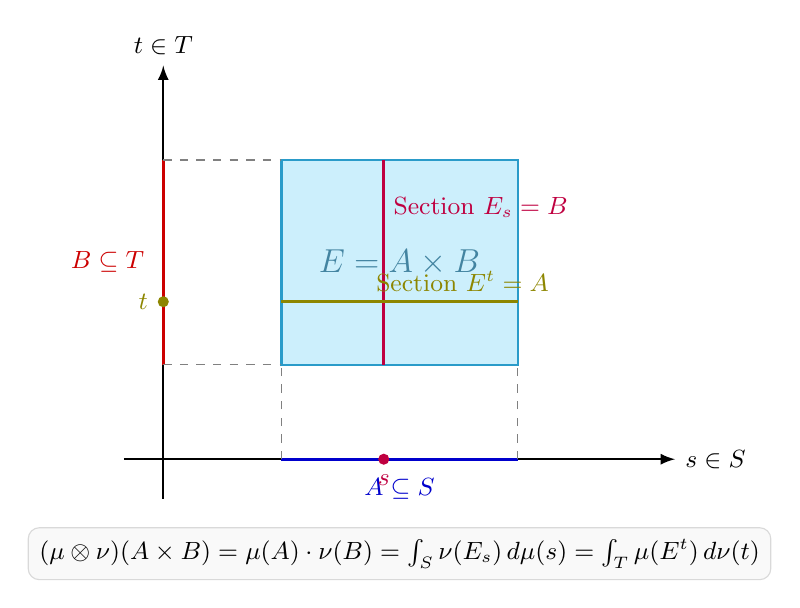
\begin{tikzpicture}[>=latex, font=\small]
  % Axes
  \draw[->, thick] (-0.5, 0) -- (6.5, 0) node[right] {$s \in S$};
  \draw[->, thick] (0, -0.5) -- (0, 5.0) node[above] {$t \in T$};

  % Rectangle A x B
  \draw[thick, fill=cyan!20, draw=cyan!80!black] (1.5, 1.2) rectangle (4.5, 3.8);
  \node[font=\large\bfseries, cyan!60!black] at (3.0, 2.5) {$E = A \times B$};

  % Projection onto S-axis
  \draw[very thick, blue!80!black] (1.5, 0) -- (4.5, 0) node[midway, below=3pt] {$A \subseteq S$};
  \draw[dashed, gray] (1.5, 0) -- (1.5, 1.2);
  \draw[dashed, gray] (4.5, 0) -- (4.5, 1.2);

  % Projection onto T-axis
  \draw[very thick, red!80!black] (0, 1.2) -- (0, 3.8) node[midway, left=3pt] {$B \subseteq T$};
  \draw[dashed, gray] (0, 1.2) -- (1.5, 1.2);
  \draw[dashed, gray] (0, 3.8) -- (1.5, 3.8);

  % Sections
  \draw[very thick, purple] (2.8, 1.2) -- (2.8, 3.8);
  \node[purple, right] at (2.8, 3.2) {Section $E_s = B$};
  \fill[purple] (2.8, 0) circle (2pt) node[below=2pt] {$s$};

  \draw[very thick, olive] (1.5, 2.0) -- (4.5, 2.0);
  \node[olive, above] at (3.8, 2.0) {Section $E^t = A$};
  \fill[olive] (0, 2.0) circle (2pt) node[left=2pt] {$t$};

  \node[align=center, fill=gray!5, draw=gray!30, rounded corners, inner sep=4pt] at (3.0, -1.2)
    {$(\mu \otimes \nu)(A \times B) = \mu(A) \cdot \nu(B) = \int_S \nu(E_s)\,d\mu(s) = \int_T \mu(E^t)\,d\nu(t)$};
\end{tikzpicture}
\end{document}
